\documentclass{article}

\usepackage{fullpage}
\usepackage{color}
\usepackage{amsmath}
\usepackage{url}
\usepackage{verbatim}
\usepackage{graphicx}
\usepackage{parskip}
\usepackage{amssymb}
\usepackage{nicefrac}
\usepackage{listings} % For displaying code
\usepackage{algorithm2e} % pseudo-code

\def\rubric#1{\gre{Rubric: \{#1\}}}{}

% Colors
\definecolor{blu}{rgb}{0,0,1}
\def\blu#1{{\color{blu}#1}}
\definecolor{gre}{rgb}{0,.5,0}
\def\gre#1{{\color{gre}#1}}
\definecolor{red}{rgb}{1,0,0}
\def\red#1{{\color{red}#1}}
\def\norm#1{\|#1\|}

% Math
\def\R{\mathbb{R}}
\def\argmax{\mathop{\rm arg\,max}}
\def\argmin{\mathop{\rm arg\,min}}
\newcommand{\mat}[1]{\begin{bmatrix}#1\end{bmatrix}}
\newcommand{\alignStar}[1]{\begin{align*}#1\end{align*}}
\def\half{\frac 1 2}

% LaTeX
\newcommand{\fig}[2]{\includegraphics[width=#1\textwidth]{#2}}
\newcommand{\centerfig}[2]{\begin{center}\includegraphics[width=#1\textwidth]{#2}\end{center}}
\def\items#1{\begin{itemize}#1\end{itemize}}
\def\enum#1{\begin{enumerate}#1\end{enumerate}}

\begin{document}


\title{CPSC 340 Assignment 5 (due Friday March 23 at 9:00pm)}
\date{}
\maketitle

\vspace{-7em}

\vspace{1em}


\section{MAP Estimation}


\[
f(w) = \frac{1}{2}\norm{Xw - y}^2 + \frac \lambda 2 \norm{w}^2.
\]

\blu{For each of the alternate assumptions below, show how the loss function would change} (simplifying as much as possible):
\enum{
\item We use a zero-mean Laplace prior for each variable with a scale parameter of $\lambda^{-1}$, so that
\[
p(w_j) = \frac{\lambda}{2}\exp(-\lambda|w_j|).
\]\\
\gre{
We're only changing the prior, so the beginning part of the function stays the same ($\frac{1}{2}\norm{Xw - y}^2$).
\\
If we take the negative log of $\frac{\lambda}{2}\exp(-\lambda|w_j|)$, it becomes $-ln(\frac{\lambda}{2}) + \lambda|w_j|$ for a given $j$.
\\
Hence, for all $j$, we get $-ln(\frac{\lambda}{2}) + \sum_{j=1}^{n}λ|w_j|$.
\\\\
Thus, the change is that we end up using L1-regularization instead of L2-regularization.
}
\item We use a Laplace likelihood with a mean of $w^Tx_i$ and a scale of $1$, so that
\[
p(y_i | x_i, w) = \frac 1 2 \exp(-|w^Tx_i - y_i|).
\]\\
\gre{
We're only changing the likelihood, so the end part of the function stays the same ($\frac \lambda 2 \norm{w}^2$).
\\
If we take the negative log of $\frac 1 2 \exp(-|w^Tx_i - y_i|)$, it becomes $-ln(\frac{1}{2}) + |w^Tx_i - y|$ for a given $i$.
\\
Hence, for all $i$, we get $-ln(\frac{1}{2}) + \sum_{i=1}^{n}|w^Tx_i - y_i|$, which is equivalent to $-ln(\frac{1}{2}) + |Xw - y|_1$.
\\\\
Thus, the change is that our data fitting term now uses the L1 norm.
}
\item We use a Gaussian likelihood where each datapoint has variance $\sigma^2$ instead of $1$,
\[
p(y_i | x_i,w) = \frac{1}{\sqrt{2\sigma^2\pi}}\exp\left(-\frac{(w^Tx_i - y_i)^2}{2\sigma^2}\right).
\]
\gre{
We're only changing the likelihood, so the end part of the function stays the same ($\frac \lambda 2 \norm{w}^2$).
\\
If we take the negative log of $p(y_i | x_i,w) = \frac{1}{\sqrt{2\sigma^2\pi}}\exp\left(-\frac{(w^Tx_i - y_i)^2}{2\sigma^2}\right)$, we get $-ln(\frac{1}{\sqrt{2\sigma^2\pi}} + \frac{(w^Tx_i - y_i)^2}{2\sigma^2}$ for a given $i$.
\\
Hence, for all $i$, we get $-ln(\frac{1}{\sqrt{2\sigma^2\pi}}) + \sum_{i=1}^{n}\frac{(w^Tx_i - y_i)^2}{2\sigma^2}$, which is equivalent to $-ln(\frac{1}{\sqrt{2\sigma^2\pi}} + \frac{||Xw-y||_2}{2\sigma^2}$.
\\\\
Thus, the change is that our data fitting term is also divided by the variance.
}
\item We use a Gaussian likelihood where each datapoint has its own variance $\sigma_i^2$,
\[
p(y_i | x_i,w) = \frac{1}{\sqrt{2\sigma_i^2\pi}}\exp\left(-\frac{(w^Tx_i - y_i)^2}{2\sigma_i^2}\right).
\]\\
\gre{
We're only changing the likelihood, so the end part of the function stays the same ($\frac \lambda 2 \norm{w}^2$).
\\
If we take the negative log of $p(y_i | x_i,w) = \frac{1}{\sqrt{2\sigma_i^2\pi}}\exp\left(-\frac{(w^Tx_i - y_i)^2}{2\sigma_i^2}\right)$, we get $-ln(\frac{1}{\sqrt{2\sigma^2_i\pi}} + \frac{(w^Tx_i - y_i)^2}{2\sigma^2}$ for a given $i$.
\\
Hence, for all $i$, we get $-ln(\frac{1}{\sqrt{2\sigma^2_i\pi}}) + \sum_{i=1}^{n}\frac{(w^Tx_i - y_i)^2}{2\sigma^2}$. 
\\
Let S be a matrix where values of $\frac{1}{2\sigma_1^2}$ to $\frac{1}{2\sigma_i^2}$ run along the main diagonal. We can then simplify the above equation to: $-ln(\frac{1}{\sqrt{2\sigma^2_i\pi}}) + (Xw - y)^TA(Xw - y)$.
\\\\
Thus, the change is that we have $n$ additional $sigma^2$ that divides the L2 norm of our data fitting term.
}
}




\section{Principal Component Analysis}

\subsection{PCA by Hand}

\blu{
\enum{
\item What is the first principal component?
\\
\gre{
The first principle component is $w_1 = (\frac{1}{\sqrt{2}},\frac{1}{\sqrt{2}})$.
}
\item What is the (L2-norm) reconstruction error of the point (3,3)? (Show your work.)
\\
\gre{
First, we want to get $z$ by subtracting by the means and multiplying by our principal component.
$$z = (3 - 0)(\frac{1}{\sqrt{2}}) + (3 - 1)(\frac{1}{\sqrt{2}}) = \frac{5}{\sqrt{2}}$$.
\\
Then, we want to get $\hat{x}$ by multiplying by our principal component and add back the means.
$$z = \frac{5}{\sqrt{2}}(\frac{1}{\sqrt{2}},\frac{1}{\sqrt{2}}) + (0, 1) = (2.5, 3.5)$$
We can get the reconstruction error like so:
$$\sqrt{(2.5 - 3)^2 + (3.5 - 3)^2}$$
$$= \frac{1}{\sqrt{2}}$$
}
\item What is the (L2-norm) reconstruction error of the point (3,4)? (Show your work.)
\\
\gre{
First, we want to get $z$ by subtracting by the means and multiplying by our principal component.
$$z = (3 - 0)(\frac{1}{\sqrt{2}}) + (4 - 1)(\frac{1}{\sqrt{2}}) = \frac{6}{\sqrt{2}}$$.
\\
Then, we want to get $\hat{x}$ by multiplying by our principal component and add back the means.
$$z = \frac{6}{\sqrt{2}}(\frac{1}{\sqrt{2}},\frac{1}{\sqrt{2}}) + (0, 1) = (3, 4)$$
We can get the reconstruction error like so:
$$\sqrt{(3 - 3)^2 + (4 - 4)^2}$$
$$= 0$$
}
}
}

\subsection{Data Visualization}

\blu{Hand in your code and the scatterplot}.

\gre{
The code can be found at $../code/main.py$.
\\
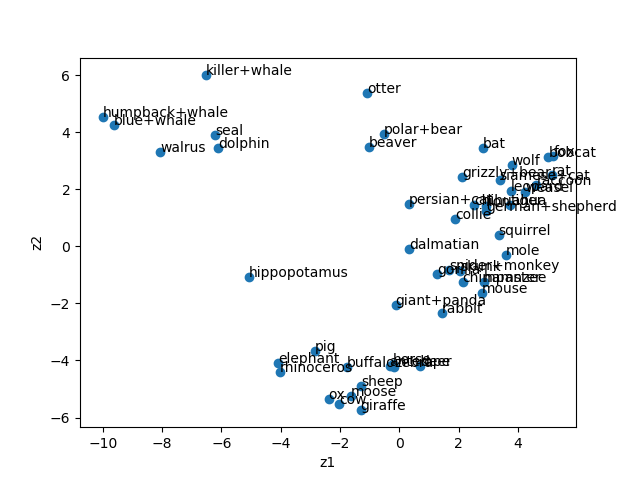
\includegraphics{../figs/q2_2_PCA_animals.png}
}
\subsection{Data Compression}

\blu{\enum{
\item How much of the variance is explained by our 2-dimensional representation from the previous question?
\\
\gre{
30.19\% of the variance is explained.
}
\item How many PCs are required to explain 50\% of the variance in the data?
\\
\gre{
We need 5 or more PCs to explain 50\% of the variance.
}
}}

\section{PCA Generalizations}

\subsection{Robust PCA}

\blu{Complete the class \emph{pca.RobustPCA},
that uses a smooth approximation to the absolute value to implement robust PCA. Comment on the quality of the results.}
\\
\gre{
The code can be found at $../code/pca.py$.
\\
The results look much better, it identifies the cars on the highway a lot better than the old version does, and the blobs of the cars moving on the highway are reduced in the background subtraction bit.
}
\section{Multi-Dimensional Scaling}

\subsection{ISOMAP}

\blu{Plot the results using $2$ and using $3$-nearest neighbours}.
\gre{
The code can be found at $../code/manifold.py$.
}
\\
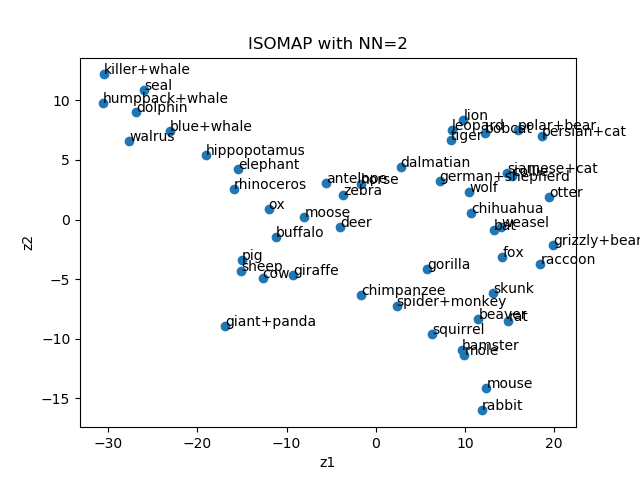
\includegraphics[scale=0.75]{../figs/q4_1_isomap_k=2.png}
\\
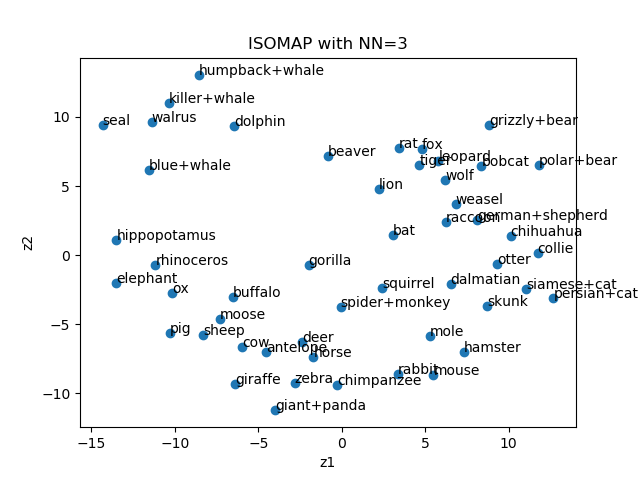
\includegraphics[scale=0.75]{../figs/q4_1_isomap_k=3.png}

\subsection{Reflection}

\blu{Briefly comment on PCA vs. MDS vs. ISOMAP for dimensionality reduction on this particular data set. In your opinion, which method did the best job and why?}
\\
\gre{
ISOMAP with k $=$ 2 seems to do the best job as it provides individual clumpings without vacuuming all the animals to one place like PCA does. MDS and ISOMAP with k = 3 don't seem to give very clear groupings of the animals and seems very general.
}

\section{Very-Short Answer Questions}

\enum{
\item Why is the kernel trick often better than explicitly transforming your features into a new space?
\\
\gre{
Because you don’t have to store the ‘Z’ and ‘w’, uses the dot product between all the training examples instead of storing the training examples themselves. Some k’s are just too large to store \- makes multi-dimensional polynomial basis intractable.
}
\item Why is the kernel trick more popular for SVMs than with logistic regression?
\\
\gre{
Kernel trick would have to process all the points in the logistic regression case, while it would only need to process the support vector examples in the case of the SVM. \- so it would be way less time consuming.
}
\item What is the key advantage of stochastic gradient methods over gradient descent methods?
\\
\gre{
Iterations are ’n’ times faster than gradient descent iterations \- because it uses the gradient of a randomly chosen training example.
}
\item Does stochastic gradient descent with a fixed $\alpha$ converge to the minimum of a convex function in general?
\\
\gre{
No, because as the points reach the confusion point \- nearer the min \- the direction of the gradient becomes confused and goes in many directions. So if you left it as the same size it would just stay in this ball (with a radius of $\alpha^t$).
}
\item What is the difference between multi-label and multi-class classification?
\\
\gre{
In multi-class there is one “label” vs. multi-label $=$ many labels where many can be correct.
}
\item What is the difference between MLE and MAP?
\\
\gre{
For MLE, we're looking for the maximizer that maximizes the likelihood.
For MAP, we're looking for the maximizer that maximizes likelihood multiplied by the prior.
}
\item Linear regression with one feature and PCA with 2 features (and $k=1$) both find a line in a two-dimensional space. Do they find the same line?
 Briefly justify your answer.
\\
\gre{
No. Linear regression tries to find a line minimizing vertical squared distance (we only care about predicting the other feature), while PCA tries to find a line that minimizes squared distance in both directions.
}
\item Are the vectors minimizing the PCA objective unique? Briefly justify your answer.
\\
\gre{
No. They are non-unique due to reasons such as ordering, scaling and rotation.
}
\item Name two methods for promoting sparse solutions in a linear regression model that result in convex problems.
\\
\gre{
Non-negative least squares, and L1 regularization.
}
\item Can we use the normal equations to solve non-negative least squares problems?
\\
\gre{
No. Solving for least squares and then setting all negative weights to 0 would be a naive solution, as you may no longer be at the best solution after setting your negative weights to 0.
}
}



\end{document}
